% Intended LaTeX compiler: pdflatex
\documentclass[10pt,a4paper,UTF8]{article}
\usepackage{zclorg}
\author{张朝龙}
\date{}
\title{学习Python Doc第四天:数据结构}
\hypersetup{
 pdfauthor={张朝龙},
 pdftitle={学习Python Doc第四天:数据结构},
 pdfkeywords={},
 pdfsubject={},
 pdfcreator={Emacs 25.0.50.1 (Org mode 9.0.5)}, 
 pdflang={English}}
\begin{document}

\maketitle
\tableofcontents
\titlepic{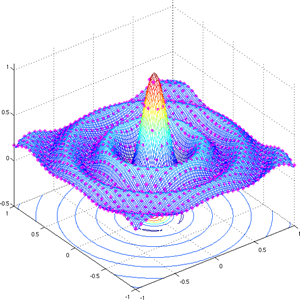
\includegraphics[scale=0.25]{../../img/sinc.PNG}}
\newpage

\texttt{Python} 提供了丰富的数据结构,极大提高编码效率。今天,我们讨论与数据结构有关的知识点。

\section{深入了解 \texttt{list}}
\label{sec:org0fffd66}


首先 \texttt{list} 数据类型提供了很多方法,我们把这些方法列举如下:
\begin{instance}
\begin{enumerate}
\item \texttt{list.append(x)} 添加一个元素到列表的尾部,等效于 \emph{a[len(a) :]=[x]} 注意等式右边的写法是 \texttt{[x]} 而不是 \texttt{x}
\item \texttt{list.extend(iterable)}  用 \texttt{iterable} 中的元素扩展 \texttt{list} ,等效于 \emph{a[len(a) :] = iterable}
\item \texttt{list.insert(i,x)}  在指定位置添加新元素。第一个输入 \texttt{i} 是插入新元素的位置, 比如 \texttt{a.insert(0,x)} 是在 \texttt{list} 的第0个位置插入 \texttt{x} , \texttt{a.insert(len(a),x)} 等效于 \texttt{a.append(x)}
\item \texttt{list.remove(x)}  从 \texttt{list} 中移除第一个 \texttt{x} ,如果 \texttt{list} 中没有 \texttt{x} 则报错
\item \texttt{list.pop([i])} 从 \texttt{list} 的指定位置删除元素,并返回这个元素。 如果没有给定具体位置,则弹出最后一个元素。注意 \texttt{[]} 表示这个函数参数是可选的。
\item \texttt{list.index(x,[start],[end])} 返回第一个 \texttt{x} 的位置。 \texttt{start} 和 \texttt{end} 表示查找 \texttt{x} 的范围。
\item \texttt{list.count(x)} 返回 \texttt{x} 在 \texttt{list} 中出现的次数
\item \texttt{list.sort(key=None,reverse=False)} 对 \texttt{list} 中的元素进行排序
\item \texttt{list.reverse()}  对  =list= 中的元素,逆序排序
\item \texttt{list.copy} 返回一个 \texttt{list} 的副本
\end{enumerate}
\end{instance}
\subsection{把 \texttt{list} 当栈用}
\label{sec:org85c0c4e}


\texttt{list} 结构以及其附带的方法,使得可以方便的把 \texttt{list} 当做栈(后进先出)用。看代码:
\begin{verbatim}
In [179]: stack = [3,4,5]

In [194]: stack.append(6)

In [198]: stack.append(7)

In [202]: stack
Out[210]: 
[3, 4, 5, 6, 7]

In [211]: stack.pop()
Out[215]: 
7

In [216]: stack
Out[220]: 
[3, 4, 5, 6]
\end{verbatim}
\subsection{把 \texttt{list} 当队列用}
\label{sec:org37badd4}


同样,也可以使用 \texttt{list} 实现队列。对立的特点是先进先出,然而 \texttt{list} 对于这个操作并不是很高效,因为从 \texttt{list} 的尾部插入元素和弹出元素比较快,但是从 \texttt{list} 的头部插入或者弹出元素比较慢(因为所有的其他元素都要移位一次)。

为了实现队列,我们使用 \texttt{collections.deque} 。 \texttt{collections.deque} 的设计使得从队列的头部和尾部插入或者弹出元素都很方便。

看代码:
\begin{verbatim}
In [221]: from collections import deque

In [234]: queue = deque(['Eric','John','Michael'])

In [265]: queue.append('Terry')

In [282]: queue.append('Grahm')

In [298]: queue
Out[298]: 
deque(['Eric', 'John', 'Michael', 'Terry', 'Grahm'])

In [299]: queue.popleft()
Out[306]: 
'Eric'

In [307]: queue.popleft()
Out[313]: 
'John'
\end{verbatim}
\subsection{队列推导式}
\label{sec:orgeddcc9d}


队列推导式提供了一种简单的创建列表的方法。当我们需要把一些运算的结果作为队列元素时,队列推导式显得非常的方便。
\begin{verbatim}
squares = []
for x in range(10):
    squares.append(x**2)
\end{verbatim}

输出:
\begin{verbatim}
In [333]: squares
Out[337]: 
[0, 1, 4, 9, 16, 25, 36, 49, 64, 81]
\end{verbatim}
当然,我们可以使用更方便的方法创建上面的这个 \texttt{list} 

\begin{verbatim}
squares = list(map(lambda x:x**2,range(10)))
\end{verbatim}
或者
\begin{verbatim}
squares = [x**2 for x in range(10)]
\end{verbatim}

列表推导式由包含一个表达式的括号组成,表达式后面跟随一个 \texttt{for} 子句,之后可以有零或多个 \texttt{for} 或 \texttt{if} 子句。结果是一个列表,由表达式依据其后面的 \texttt{for} 和 \texttt{if} 子句上下文计算而来的结果构成。

比如
\begin{verbatim}
In [339]: [(x,y) for x in [1,2,3] for y in [3,1,4] if x!=y]
Out[397]: 
[(1, 3), (1, 4), (2, 3), (2, 1), (2, 4), (3, 1), (3, 4)]
\end{verbatim}
上面的一行代码等效于:
\lstset{language=Python,label= ,caption= ,captionpos=b,firstnumber=1,numbers=left}
\begin{lstlisting}
comp = []
for x in [1,2,3]:
    for y in [3,1,4]:
        if x != y:
            comp.append((x,y))
\end{lstlisting}
我们再给几个例子:
\begin{verbatim}
In [399]: vec = [-4,-2,0,2,4]

In [409]: [x*2 for x in vec]
Out[416]: 
[-8, -4, 0, 4, 8]

In [417]: [x for x in vec if x>=0]
Out[444]: 
[0, 2, 4]

In [445]: [abs(x) for x in vec]
Out[456]: 
[4, 2, 0, 2, 4]

In [457]: freshfruit = [' banana',' loganberry','passion fruit ']

In [506]: [weapon.strip() for weapon in freshfruit]
Out[536]: 
['banana', 'loganberry', 'passion fruit']

In [537]: [(x,x**2) for x in range(6)]
Out[562]: 
[(0, 0), (1, 1), (2, 4), (3, 9), (4, 16), (5, 25)]

In [563]: [x,x**2 for x in range(6)]
  File "<ipython-input-563-8d6940458683>", line 1
    [x,x**2 for x in range(6)]
              ^
SyntaxError: invalid syntax


In [564]: vec = [[1,2,3],[4,5,6],[7,8,9]]

In [581]: [num for elem in vec for num in elem]
Out[596]: 
[1, 2, 3, 4, 5, 6, 7, 8, 9]
\end{verbatim}
从上面的例子,我们可以看到,如果生成的 \texttt{list} 中元素都是二元组的话,则必须用括号包起来。

\texttt{list} 生成器可以包括复杂的表达式或者嵌套函数

\begin{verbatim}
In [602]: [str(round(pi,i)) for i in range(1,6)]
Out[616]: 
['3.1', '3.14', '3.142', '3.1416', '3.14159']
\end{verbatim}
\subsection{嵌套的 \texttt{list} 推导式}
\label{sec:orgd2b4013}


\texttt{list} 推导式的第一个表达式可以是任何表达式,包括 \texttt{list} 推导式。
\lstset{language=Python,label= ,caption= ,captionpos=b,numbers=none}
\begin{lstlisting}
matrix = [
    [1,2,3,4],
    [5,6,7,8],
    [9,10,11,12],
]
[[row[i] for row in matrix] for i in range(4)]
\end{lstlisting}
输出为:
\begin{verbatim}
In [619]: [[row[i] for row in matrix] for i in range(4)]
Out[658]: 
[[1, 5, 9], [2, 6, 10], [3, 7, 11], [4, 8, 12]]
\end{verbatim}
上面的代码实现了矩阵转置功能(交换了矩阵的行和列)。对于 \texttt{matrix} 这样的数据结构,
\begin{verbatim}
[x[0] for x in matrix]
\end{verbatim}
输出的是 \texttt{matrix} 的第 \texttt{0} 列 \texttt{[1,5,9]} 。
整个矩阵转换代码等效于:
\lstset{language=Python,label= ,caption= ,captionpos=b,numbers=none}
\begin{lstlisting}
matrix = [
    [1,2,3,4],
    [5,6,7,8],
    [9,10,11,12],
]
transpose = []
for i in range(4):
    transpose.append([row[i] for row in matrix])
\end{lstlisting}
鉴于 \texttt{Python} 强大的函数库,这个转置功能可以通过 \texttt{zip} 来实现。
\begin{verbatim}
list(zip(*matrix))
\end{verbatim}
输出是:
\begin{verbatim}
[(1, 5, 9), (2, 6, 10), (3, 7, 11), (4, 8, 12)]
\end{verbatim}
\section{\texttt{del} 语句}
\label{sec:org27dc559}


\texttt{list.remove(x)} 删除 \texttt{list} 中第一个值为 \texttt{x} 的元素。在移除的过程中必须给定 \texttt{x} 。  使用 \texttt{del} 语句可以不用给定 \texttt{x} 只用给定索引号就删除指定位置的元素。

\begin{verbatim}
In [736]: a = [1,2,3,4,5,6,7]

In [758]: del a[0]

In [770]: a
Out[770]: 
[2, 3, 4, 5, 6, 7]

In [771]: del a[5]

In [787]: a
Out[787]: 
[2, 3, 4, 5, 6]

In [788]: del a[2]

In [792]: a
Out[792]: 
[2, 3, 5, 6]
\end{verbatim}

\texttt{del} 也可以用来删除一个变量
\begin{verbatim}
del a
\end{verbatim}

\section{\texttt{tuple} 和 \texttt{sequence}}
\label{sec:orgb4afeaf}


\texttt{list} 和 \texttt{strings} 是两个 \texttt{sequence} 类型的数据类型。由于 \texttt{Python} 是一个不断演进的语言, \texttt{tuple} 是新加入的 \texttt{sequence} 成员。一个 \texttt{tuple} 的成员用逗号隔开,看例子:
\begin{verbatim}
In [793]: t = 12345, 54321, 'hello!'

In [821]: t[0]
Out[828]: 
12345

In [829]: t[2]
Out[832]: 
'hello!'

In [833]: t
Out[837]: 
(12345, 54321, 'hello!')

In [838]: u = t,(1,3,4)

In [854]: u
Out[854]: 
((12345, 54321, 'hello!'), (1, 3, 4))

In [855]: t[0]
Out[863]: 
12345

In [864]: t[0] = 8888
---------------------------------------------------------------------------
TypeError                                 Traceback (most recent call last)
<ipython-input-871-7f2f230bad03> in <module>()
----> 1 t[0] = 8888

TypeError: 'tuple' object does not support item assignment

In [872]: v = ([1,2,3],[4,5,6])

In [887]: v
Out[887]: 
([1, 2, 3], [4, 5, 6])
\end{verbatim}

从上面例子可以看出, \texttt{tuple} 的输出总是有括号包括。不可以给 \texttt{tuple} 中单个元素赋值。

尽管 \texttt{tuple} 和 \texttt{list} 有很多相似之处,但是他们经常在不同的场合使用。 \texttt{tuple} 是不可修改的。通常 \texttt{tuple} 包含不同种类的成员。 \texttt{list} 的成员则通常是相同类型的并可以通过迭代读写。

在创建另个或者一个元素的 \texttt{tuple} 时,有一些简单的技巧。
\begin{verbatim}
In [888]: empty = ()

In [903]: singleton = 'hello', # note the trailing comma

In [920]: len(empty)
Out[920]: 
0

In [921]: len(singleton)
Out[933]: 
1

In [934]: singleton
Out[942]: 
('hello',)
\end{verbatim}

\section{\texttt{set}}
\label{sec:org2b91b4b}


\texttt{Python} 还有一个数据类型 \texttt{set} . 一个 \texttt{set} 是一组无重复元素的集合。 \texttt{set} 支持数学概念上的 \texttt{并} \texttt{交} \texttt{差} \texttt{对称差} . 通常用花括号和 \texttt{set()} 来创建 \texttt{set}

\begin{verbatim}
In [943]: basket = {'apple','orange','apple','pear','orange','banana'}

In [989]: print(basket)
{'banana', 'orange', 'pear', 'apple'}
\end{verbatim}
可以看出 \texttt{set} 自动删除集合中的重复元素。
\begin{verbatim}
In [997]: 'orange' in basket #fast membership testing
Out[1027]: 
True

In [1028]: 'crabgrass' in basket
Out[1052]: 
False
\end{verbatim}

可以快速的进行成员验证。

\begin{verbatim}
In [1053]: a = set('abracadabra')

In [1066]: b = set('alacazam')

In [1078]: a
Out[1078]: 
{'a', 'b', 'c', 'd', 'r'}

In [1079]: b
Out[1083]: 
{'a', 'c', 'l', 'm', 'z'}

In [1084]: a-b # letters in a but not in b
Out[1091]: 
{'b', 'd', 'r'}

In [1092]: a | b #letters in either a or b
Out[1099]: 
{'a', 'b', 'c', 'd', 'l', 'm', 'r', 'z'}

In [1100]: a + b #do not support +
---------------------------------------------------------------------------
TypeError                                 Traceback (most recent call last)
<ipython-input-1100-f96fb8f649b6> in <module>()
----> 1 a + b

TypeError: unsupported operand type(s) for +: 'set' and 'set'

In [1101]: a & b #letter in both a and b
Out[1108]: 
{'a', 'c'}

In [1109]: a ^ b #letters in a or b nut not both
Out[1120]: 
{'b', 'd', 'l', 'm', 'r', 'z'}
\end{verbatim}

\texttt{Python} 除了支持列表推导式外,也支持集合推导式。
\begin{verbatim}
In [1121]: a = {x for x in 'abracadabra' if x not in 'abc'}

In [1146]: a
Out[1146]: 
{'d', 'r'}
\end{verbatim}

\section{字典(dictionaries)}
\label{sec:org5817950}


\texttt{dictionary} 是 \texttt{Python} 支持的又一数据类型,这个数据类型不是序列类型,而是映射类型(mapping types)。 序列类型( \texttt{list} \texttt{tuple} \texttt{set} )通过数字来索引元素, 映射类型的数据通过 关键字 (key)来索引元素。字符创和数字可以当做 \texttt{key} 来使用。如果 \texttt{tuple} 的成员都是 字符创,数字或者 \texttt{tuple} ,那么 \texttt{tuple} 也可以用来当做 \texttt{key} . 不能用 \texttt{list} 来当做 \texttt{key} ,因为 \texttt{list} 能够被修改。

通常,我们可以想象字典是一系列没有排序的 \texttt{key:value}  对,其中 \texttt{key} 在一个字典中是唯一的。 \texttt{\{\}} 创建空的字典。在字典中我们经常用的操作是按照某个 \texttt{key} 保存一个 \texttt{value} 或者,根据某个 \texttt{key} 读取 \texttt{value} 。同样,我们可以使用 \texttt{del} 来删除 \texttt{key:value} 。如果新存入的 \texttt{key} 和原来重复,那么原来的 \texttt{key} 对应的 \texttt{value} 就会被覆盖。如果试图从字典中读取某个不存在的 \texttt{key} 对应的 \texttt{value} 那么报错。

对一个字典执行 \texttt{list(d.keys())} 操作,返回这个字典使用的所有 \texttt{key} ,返回的 \texttt{list} 是无序的,如果你需要返回结果有序,那么使用 \texttt{sorted(d.keys())} . 使用 \texttt{in} 进行成员关系测试。看代码:
\begin{verbatim}
In [1147]: tel = {'jack':4098, 'sape':4139}

In [1186]: tel['guido'] = 4127

In [1198]: tel
Out[1198]: 
{'guido': 4127, 'jack': 4098, 'sape': 4139}

In [1199]: tel['jack']
Out[1211]: 
4098

In [1212]: del tel['sape']

In [1224]: tel['irv'] = 4127

In [1251]: tel
Out[1255]: 
{'guido': 4127, 'irv': 4127, 'jack': 4098}

In [1256]: list(tel.keys())
Out[1276]: 
['jack', 'irv', 'guido']

In [1277]: sorted(tel.keys())
Out[1284]: 
['guido', 'irv', 'jack']

In [1285]: 'guido' in tel
Out[1293]: 
True

In [1294]: 'jack' not in tel
Out[1300]: 
False
\end{verbatim}

可以使用 \texttt{dict()} 函数创建字典,看代码:
\begin{verbatim}
In [1301]: dict([('sape',4139),('guido',4127),('jack',4098)])
Out[1354]: 
{'guido': 4127, 'jack': 4098, 'sape': 4139}
\end{verbatim}

当然,字典也支持字典推导式,看代码:
\begin{verbatim}
In [1355]: {x:x**2 for x in (2,4,6)}
Out[1377]: 
{2: 4, 4: 16, 6: 36}
\end{verbatim}
当 \texttt{key} 是简单的字符创时,使用 \texttt{dict()} 来构建字典更容易,看代码:
\begin{verbatim}
In [1378]: dict(sape=4139,guido=4127,jack=4098)
Out[1433]: 
{'guido': 4127, 'jack': 4098, 'sape': 4139}
\end{verbatim}

\section{使用循环}
\label{sec:orgec395cc}


当在字典中使用循环的时候,可以使用 \texttt{item()} 来获取 \texttt{key:value} 。
\begin{verbatim}
knights = {'gallahad':'the pure','robin':'the brave'}
for k,v in knights.items():
    print(k,v)
\end{verbatim}

在我的环境中输出是:
\begin{verbatim}
In [1435]: robin the brave
gallahad the pure
\end{verbatim}
不知道为什么先输出了第二个 \texttt{key:value} ,难道输出是乱序的么?

当循环对象是序列类型的数据类型时,可以使用 \texttt{enumerate()} 来生成索引和该索引对应的值:
\lstset{language=Python,label= ,caption= ,captionpos=b,numbers=none}
\begin{lstlisting}
for i,v in enumerate(['tic','tac','toe']):
    print(i,v)
\end{lstlisting}
输出为:
\begin{verbatim}
In [1436]: 0 tic
1 tac
2 toe
\end{verbatim}

在两个或者多个序列( \texttt{sequence} ) 中执行循环,可以使用 \texttt{zip()} 实现。
\lstset{language=Python,label= ,caption= ,captionpos=b,numbers=none}
\begin{lstlisting}
questions = ['name','quest','favorite color']
answers = ['lancelot','the holy grail','blue']
for q,a in zip(questions,answers):
    print('what is your {0} It is {1}.'.format(q,a))
\end{lstlisting}
输出为:
\begin{verbatim}
In [1437]: what is your name It is lancelot.
what is your quest It is the holy grail.
what is your favorite color It is blue.
\end{verbatim}

其中 \texttt{list(zip(questions,answers))} 的结果是:
\begin{verbatim}
In [1438]: list(zip(questions,answers))
Out[1456]: 
[('name', 'lancelot'), ('quest', 'the holy grail'), ('favorite color', 'blue')]
\end{verbatim}
如果要对一个 \texttt{sequence} 类型的数据进行逆向循环时,使用 \texttt{reversed()} 函数。

\begin{verbatim}
for i in reversed(range(1,10,2)):
    print(i)
\end{verbatim}
输出是:
\begin{verbatim}
In [1457]: 9
7
5
3
1
\end{verbatim}
\end{document}
